\section{Experimental Results and Analysis}
\label{sec:results}
This section presents a comprehensive analysis of our benchmarking study comparing the performance of $\alpha, \beta$-CROWN and Marabou in verifying neural network controllers for autonomous driving. We evaluated four distinct neural network models of varying complexity (991, 2649, 5160, and 10018 parameters) across four robustness properties (p1, p2, p3, and p4) with perturbation bounds ($\varepsilon$) ranging from 0 to 10/255.

\begin{table}[ht]
    \centering
    \caption{Safety properties investigated.  A violation renders the input \textit{UNSAFE}.\label{tab:prop-defs}}
    \begin{tabular}{clp{0.6\linewidth}}
        \toprule
        Tag & Name & Informal description \\ \midrule
        $\mathbf{p_1}$ & Classification Robustness (CR) & The predicted manoeuvre (left/straight/right) must remain unchanged within the $\varepsilon$\,\slash\,255 $\ell_\infty$ neighbourhood. \\[2pt]
        $\mathbf{p_2}$ & Strong Classification Robustness (SCR) & The logit of the correct class must remain above a threshold $\delta_{\text{conf}}$; here the threshold is taken as a fraction of the clean logit value. \\[2pt]
        $\mathbf{p_3}$ & Combined Robustness (CR $\wedge$ SCR) & \textit{Both} conditions must hold: the class must stay unchanged \emph{and} the correct-class logit must satisfy the confidence floor. A violation of either sub-property renders the input \textit{UNSAFE}. \\[2pt]
        $\mathbf{p_4}$ & Logit Stability (all-class bound) & Every logit must remain within $\pm\,\delta_{\text{stab}}$ of its clean value, providing coordinate-wise bounded sensitivity. \\ 
        \bottomrule
    \end{tabular}
\end{table}

\subsection{Baseline Model Quality}\label{subsec:training}
Figure~\ref{fig:training-metrics-all} illustrates that all models converge rapidly, with training stabilising by epoch12. As shown in Table~\ref{tab:val-acc}, both training and validation accuracies remain consistently high across models, with validation accuracies differing by less than two percentage points. These results suggest that subsequent differences in verification performance are driven by architectural complexity rather than disparities in predictive accuracy.


\begin{table}[ht]
    \centering
    \caption{Training and validation  accuracy after 12~epochs.\label{tab:val-acc}}
    \begin{tabular}{|l|c|c|c|c|}
        \hline
        & \multicolumn{4}{c|}{Parameter count} \\ \cline{2-5}
        Metric & 991 & 2649 & 5160 & 10018 \\ \hline
        Training accuracy  (\%)   & 95.29 & 96.20 & 96.92 & 96.56 \\ \hline
        Validation accuracy (\%) & 92.3 & 93.8 & 93.8 & 92.3 \\ \hline
        
    \end{tabular}
\end{table}

%%%%%%%%%%%%%%%%%%%%%%%%%%%%%%%%%%%%%%%%%%%%%%%%%%%
\begin{figure}[ht]
    \centering
    % First row
    \begin{minipage}{0.49\linewidth}
        \centering
        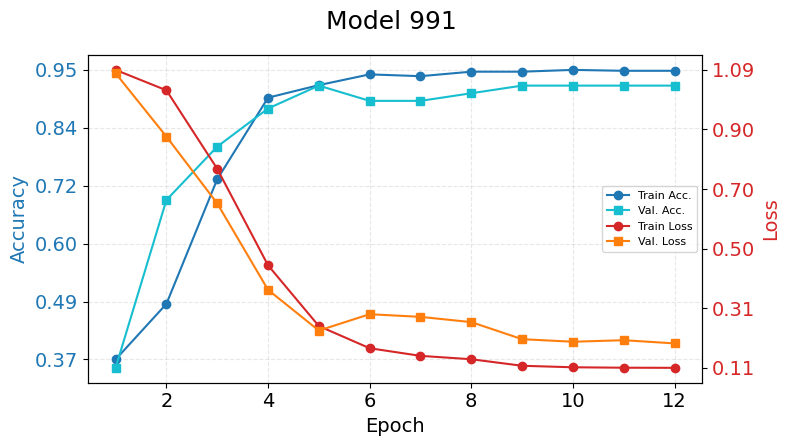
\includegraphics[width=\linewidth]{figures/train_metrics991.png}
 
    \end{minipage}
    \hfill
    \begin{minipage}{0.49\linewidth}
        \centering
        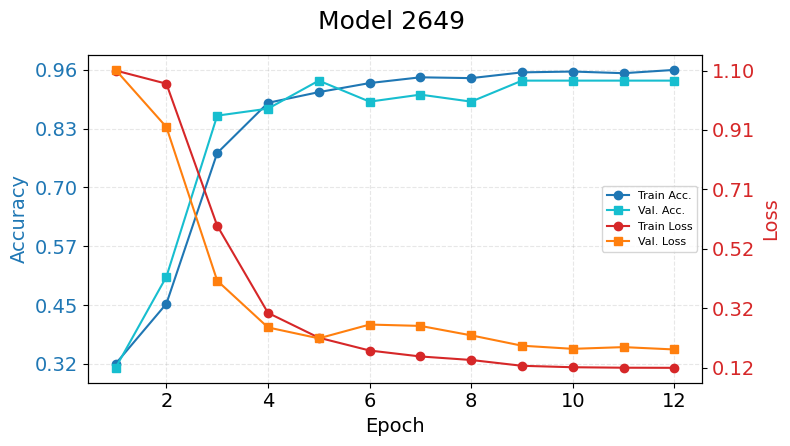
\includegraphics[width=\linewidth]{figures/train_metrics2649.png}

    \end{minipage}
    
    \vspace{0.5em} % Space between rows



    % Second row
    \begin{minipage}{0.49\linewidth}
        \centering
        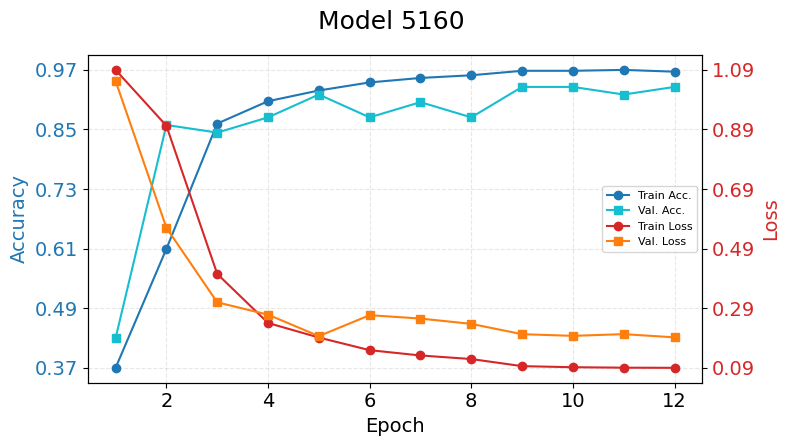
\includegraphics[width=\linewidth]{figures/train_metrics5160.png}

    \end{minipage}
    \hfill
    \begin{minipage}{0.49\linewidth}
        \centering
        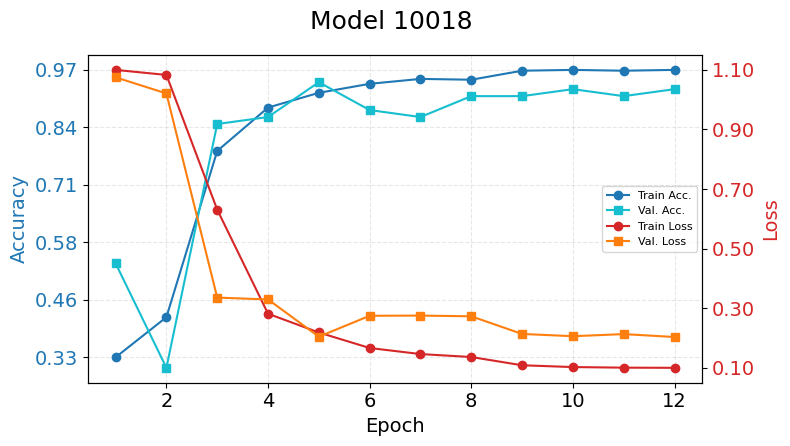
\includegraphics[width=\linewidth]{figures/train_metrics10018.png}

    \end{minipage}
    \caption{Training and validation accuracy/loss curves over 12 epochs for four model sizes. Accuracy is plotted on the left Y-axis and loss on the right Y-axis in each plot.}
    \label{fig:training-metrics-all}
\end{figure}

\subsection{Verification Outcomes Across Models and Properties}

Figure~\ref{fig:safe_unsafe_model2649_p1} shows a representative example of the verification outcomes for Model 2649 and Property p1 (Standard Robustness). The side-by-side comparison reveals that both tools provide similar results at lower perturbation bounds but diverge as the perturbation bound increases. At $\varepsilon = 6/255$, Marabou reports more "Unknown" results than $\alpha, \beta$-CROWN, indicating a difference in completeness between the two tools.

\begin{figure}[htbp]
    \centering
    \includegraphics[width=\textwidth]{figures/safe_unsafe_model2649_p1.png}
    \caption{SAFE/UNSAFE comparison for Model 2649, Property p1 (Standard Robustness). Left: $\alpha, \beta$-CROWN; Right: Marabou.}
    \label{fig:safe_unsafe_model2649_p1}
\end{figure}

Table~\ref{tab:comprehensive_summary} provides a comprehensive summary of the verification results across all models and properties. For each property and perturbation bound, we report the percentage of instances where the property was proven to hold (SAFE), violated (UNSAFE), or could not be determined within the time limit (Unknown), along with the average verification time in seconds.

\begin{table}[htbp]
\centering
\caption{Comprehensive Summary of Verification Results}
\label{tab:comprehensive_summary}
\resizebox{\textwidth}{!}{
\begin{tabular}{|l|c|c|c|c|c|c|c|c|c|}
\hline
\multirow{2}{*}{Property} & \multirow{2}{*}{$\varepsilon$} & \multicolumn{4}{c|}{$\alpha,\beta$-CROWN} & \multicolumn{4}{c|}{Marabou} \\ \cline{3-10}
 & & SAFE (\%) & UNSAFE (\%) & Unknown (\%) & Avg. Time (s) & SAFE (\%) & UNSAFE (\%) & Unknown (\%) & Avg. Time (s) \\ \hline
\multirow{5}{*}{Standard Robustness (p1)} & 0/255 & 93.1 & 6.9 & 0.0 & 2.29 & 93.1 & 6.9 & 0.0 & 4.57 \\ 
  & 1/255 & 85.8 & 14.2 & 0.0 & 3.80 & 85.8 & 14.2 & 0.0 & 35.31 \\ 
  & 3/255 & 63.8 & 33.8 & 2.3 & 9.22 & 58.5 & 33.5 & 8.1 & 281.91 \\ 
  & 6/255 & 28.8 & 69.6 & 1.5 & 12.12 & 21.9 & 62.3 & 15.8 & 499.88 \\ 
  & 10/255 & 1.5 & 98.5 & 0.0 & 12.93 & 1.2 & 89.2 & 9.6 & 400.28 \\ \hline
\hline
\multirow{5}{*}{Confidence Robustness (p2)} & 0/255 & 100.0 & 0.0 & 0.0 & 2.07 & 100.0 & 0.0 & 0.0 & 2.51 \\ 
  & 1/255 & 83.5 & 15.8 & 0.8 & 5.87 & 81.5 & 15.4 & 3.1 & 103.34 \\ 
  & 3/255 & 3.8 & 95.4 & 0.8 & 13.63 & 3.5 & 95.0 & 1.5 & 175.23 \\ 
  & 6/255 & 0.0 & 100.0 & 0.0 & 12.83 & 0.0 & 100.0 & 0.0 & 145.21 \\ 
  & 10/255 & 0.0 & 100.0 & 0.0 & 12.25 & 0.0 & 100.0 & 0.0 & 163.09 \\ \hline
\hline
\multirow{5}{*}{Combined Robustness (p3)} & 0/255 & 93.1 & 6.9 & 0.0 & 2.39 & 93.1 & 6.9 & 0.0 & 4.56 \\ 
  & 1/255 & 79.2 & 20.0 & 0.8 & 6.25 & 77.7 & 19.2 & 3.1 & 113.53 \\ 
  & 3/255 & 3.8 & 95.4 & 0.8 & 13.30 & 3.5 & 94.2 & 2.3 & 218.06 \\ 
  & 6/255 & 0.0 & 100.0 & 0.0 & 12.77 & 0.0 & 100.0 & 0.0 & 181.78 \\ 
  & 10/255 & 0.0 & 100.0 & 0.0 & 12.04 & 0.0 & 100.0 & 0.0 & 180.64 \\ \hline
\hline
\multirow{5}{*}{Logit Stability (p4)} & 0/255 & 100.0 & 0.0 & 0.0 & 2.46 & 100.0 & 0.0 & 0.0 & 2.51 \\ 
  & 1/255 & 23.5 & 75.0 & 1.5 & 11.81 & 23.8 & 71.9 & 4.2 & 234.49 \\ 
  & 3/255 & 5.4 & 94.6 & 0.0 & 10.81 & 5.4 & 93.1 & 1.5 & 195.75 \\ 
  & 6/255 & 0.4 & 99.6 & 0.0 & 9.22 & 0.4 & 97.3 & 2.3 & 201.50 \\ 
  & 10/255 & 0.0 & 100.0 & 0.0 & 7.54 & 0.0 & 98.8 & 1.2 & 186.59 \\ 
\hline
\end{tabular}
}
\end{table}


\subsection{Analysis by Property}

\subsubsection{Property p1 (Standard Robustness)}

Property p1 verifies that no misclassification occurs within the $\varepsilon$-ball around the input. As shown in Figure~\ref{fig:safe_unsafe_model991_p1}, both tools demonstrate similar verification capabilities at lower perturbation bounds but diverge significantly at higher values.

\begin{figure}[htbp]
    \centering
    \includegraphics[width=\textwidth]{figures/safe_unsafe_model991_p1.png}
    \caption{SAFE/UNSAFE comparison for Model 991, Property p1 (Standard Robustness). Left: $\alpha, \beta$-CROWN; Right: Marabou.}
    \label{fig:safe_unsafe_model991_p1}
\end{figure}

The verification time for Property p1 also varies significantly between the two tools, as shown in Figure~\ref{fig:time_model991_p1}. $\alpha, \beta$-CROWN consistently outperforms Marabou in terms of efficiency, especially at higher perturbation bounds.

\begin{figure}[htbp]
    \centering
    \includegraphics[width=\textwidth]{figures/time_model991_p1.png}
    \caption{Verification time comparison for Model 991, Property p1 (Standard Robustness). Left: $\alpha, \beta$-CROWN; Right: Marabou.}
    \label{fig:time_model991_p1}
\end{figure}

At $\varepsilon = 0/255$ (unperturbed inputs), both tools correctly verify that approximately 92\% of instances satisfy the property. As $\varepsilon$ increases to 3/255, $\alpha, \beta$-CROWN maintains a higher rate of definitive results compared to Marabou, with Marabou reporting more instances as "Unknown." This gap widens at $\varepsilon = 6/255$, where Marabou cannot determine the outcome for a significant number of instances.

Table~\ref{tab:p1_tool_comparison} provides a detailed comparison of the two tools for Property p1 across all models and perturbation bounds.

\begin{table}[htbp]
\centering
\caption{Tool Comparison for Standard Robustness (p1)}
\label{tab:p1_tool_comparison}
\begin{tabular}{|c|c|c|c|c|c|c|c|c|c|}
\hline
\multirow{2}{*}{Model} & \multirow{2}{*}{$\varepsilon$} & \multicolumn{4}{c|}{$\alpha,\beta$-CROWN} & \multicolumn{4}{c|}{Marabou} \\ \cline{3-10}
 & & SAFE & UNSAFE & Unknown & Time (s) & SAFE & UNSAFE & Unknown & Time (s) \\ \hline
\multirow{5}{*}{991} & 0/255 & 60 & 5 & 0 & 2.03 & 60 & 5 & 0 & 3.51 \\ 
  & 1/255 & 56 & 9 & 0 & 3.42 & 56 & 9 & 0 & 24.50 \\ 
  & 3/255 & 42 & 21 & 2 & 8.57 & 39 & 21 & 5 & 228.58 \\ 
  & 6/255 & 18 & 45 & 2 & 12.26 & 16 & 39 & 10 & 421.71 \\ 
  & 10/255 & 1 & 64 & 0 & 13.55 & 1 & 57 & 7 & 365.88 \\ \hline
\hline
\multirow{5}{*}{2649} & 0/255 & 61 & 4 & 0 & 2.07 & 61 & 4 & 0 & 3.99 \\ 
  & 1/255 & 55 & 10 & 0 & 4.40 & 55 & 10 & 0 & 35.07 \\ 
  & 3/255 & 42 & 23 & 0 & 7.41 & 42 & 23 & 0 & 114.16 \\ 
  & 6/255 & 18 & 47 & 0 & 11.27 & 14 & 46 & 5 & 334.82 \\ 
  & 10/255 & 1 & 64 & 0 & 12.24 & 1 & 61 & 3 & 301.34 \\ \hline
\hline
\multirow{5}{*}{5160} & 0/255 & 61 & 4 & 0 & 2.55 & 61 & 4 & 0 & 4.70 \\ 
  & 1/255 & 56 & 9 & 0 & 3.71 & 56 & 9 & 0 & 35.46 \\ 
  & 3/255 & 40 & 22 & 3 & 10.88 & 36 & 22 & 7 & 369.54 \\ 
  & 6/255 & 19 & 45 & 1 & 11.45 & 15 & 39 & 11 & 545.60 \\ 
  & 10/255 & 1 & 64 & 0 & 12.18 & 1 & 57 & 7 & 387.73 \\ \hline
\hline
\multirow{5}{*}{10018} & 0/255 & 60 & 5 & 0 & 2.51 & 60 & 5 & 0 & 6.07 \\ 
  & 1/255 & 56 & 9 & 0 & 3.68 & 56 & 9 & 0 & 46.23 \\ 
  & 3/255 & 42 & 22 & 1 & 10.01 & 35 & 21 & 9 & 415.35 \\ 
  & 6/255 & 20 & 44 & 1 & 13.51 & 12 & 38 & 15 & 697.39 \\ 
  & 10/255 & 1 & 64 & 0 & 13.77 & 0 & 57 & 8 & 546.18 \\ 
\hline
\end{tabular}
\end{table}


\subsubsection{Property p2 (Confidence Robustness)}

Property p2 ensures that class confidence remains above a threshold within the perturbation bound. As illustrated in Figure~\ref{fig:safe_unsafe_model991_p2}, both tools show similar verification patterns but with significant differences in efficiency.

\begin{figure}[htbp]
    \centering
    \includegraphics[width=\textwidth]{figures/safe_unsafe_model991_p2.png}
    \caption{SAFE/UNSAFE comparison for Model 991, Property p2 (Confidence Robustness). Left: $\alpha, \beta$-CROWN; Right: Marabou.}
    \label{fig:safe_unsafe_model991_p2}
\end{figure}

The verification time comparison for Property p2 is shown in Figure~\ref{fig:time_model991_p2}, highlighting the efficiency advantage of $\alpha, \beta$-CROWN over Marabou.

\begin{figure}[htbp]
    \centering
    \includegraphics[width=\textwidth]{figures/time_model991_p2.png}
    \caption{Verification time comparison for Model 991, Property p2 (Confidence Robustness). Left: $\alpha, \beta$-CROWN; Right: Marabou.}
    \label{fig:time_model991_p2}
\end{figure}

At $\varepsilon = 0/255$, both tools verify that 100\% of instances satisfy the property. As $\varepsilon$ increases to 1/255, $\alpha, \beta$-CROWN determines outcomes for more instances than Marabou. At $\varepsilon = 3/255$, both tools find that the property is violated in most cases, indicating that confidence drops significantly even with small perturbations.

Table~\ref{tab:p2_tool_comparison} provides a detailed comparison of the two tools for Property p2 across all models and perturbation bounds.

\begin{table}[htbp]
\centering
\caption{Tool Comparison for Confidence Robustness (p2)}
\label{tab:p2_tool_comparison}
\begin{tabular}{|c|c|c|c|c|c|c|c|c|c|}
\hline
\multirow{2}{*}{Model} & \multirow{2}{*}{$\varepsilon$} & \multicolumn{4}{c|}{$\alpha,\beta$-CROWN} & \multicolumn{4}{c|}{Marabou} \\ \cline{3-10}
 & & SAFE & UNSAFE & Unknown & Time (s) & SAFE & UNSAFE & Unknown & Time (s) \\ \hline
\multirow{5}{*}{991} & 0/255 & 65 & 0 & 0 & 2.18 & 65 & 0 & 0 & 1.95 \\ 
  & 1/255 & 61 & 4 & 0 & 3.95 & 60 & 3 & 2 & 76.42 \\ 
  & 3/255 & 4 & 59 & 2 & 16.34 & 3 & 59 & 3 & 199.01 \\ 
  & 6/255 & 0 & 65 & 0 & 13.32 & 0 & 65 & 0 & 84.43 \\ 
  & 10/255 & 0 & 65 & 0 & 13.14 & 0 & 65 & 0 & 95.87 \\ \hline
\hline
\multirow{5}{*}{2649} & 0/255 & 65 & 0 & 0 & 1.92 & 65 & 0 & 0 & 2.23 \\ 
  & 1/255 & 56 & 9 & 0 & 4.46 & 56 & 9 & 0 & 35.86 \\ 
  & 3/255 & 0 & 65 & 0 & 13.31 & 0 & 65 & 0 & 121.91 \\ 
  & 6/255 & 0 & 65 & 0 & 13.36 & 0 & 65 & 0 & 117.15 \\ 
  & 10/255 & 0 & 65 & 0 & 12.78 & 0 & 65 & 0 & 131.40 \\ \hline
\hline
\multirow{5}{*}{5160} & 0/255 & 65 & 0 & 0 & 2.07 & 65 & 0 & 0 & 2.64 \\ 
  & 1/255 & 51 & 13 & 1 & 5.65 & 51 & 13 & 1 & 75.18 \\ 
  & 3/255 & 4 & 61 & 0 & 12.29 & 4 & 60 & 1 & 172.36 \\ 
  & 6/255 & 0 & 65 & 0 & 12.37 & 0 & 65 & 0 & 156.01 \\ 
  & 10/255 & 0 & 65 & 0 & 11.78 & 0 & 65 & 0 & 165.60 \\ \hline
\hline
\multirow{5}{*}{10018} & 0/255 & 65 & 0 & 0 & 2.12 & 65 & 0 & 0 & 3.22 \\ 
  & 1/255 & 49 & 15 & 1 & 9.42 & 45 & 15 & 5 & 225.88 \\ 
  & 3/255 & 2 & 63 & 0 & 12.58 & 2 & 63 & 0 & 207.65 \\ 
  & 6/255 & 0 & 65 & 0 & 12.29 & 0 & 65 & 0 & 223.25 \\ 
  & 10/255 & 0 & 65 & 0 & 11.28 & 0 & 65 & 0 & 259.49 \\ 
\hline
\end{tabular}
\end{table}


\subsubsection{Property p3 (Combined Robustness)}

Property p3 requires either no misclassification or confidence to remain high. As shown in Figure~\ref{fig:safe_unsafe_model991_p3}, this property shows verification patterns similar to the confidence robustness property (p2), suggesting that the confidence threshold is the dominant factor in this combined property.

\begin{figure}[htbp]
    \centering
    \includegraphics[width=\textwidth]{figures/safe_unsafe_model991_p3.png}
    \caption{SAFE/UNSAFE comparison for Model 991, Property p3 (Combined Robustness). Left: $\alpha, \beta$-CROWN; Right: Marabou.}
    \label{fig:safe_unsafe_model991_p3}
\end{figure}

Figure~\ref{fig:time_model991_p3} shows the verification time comparison for Property p3, which follows a similar pattern to the other properties.

\begin{figure}[htbp]
    \centering
    \includegraphics[width=\textwidth]{figures/time_model991_p3.png}
    \caption{Verification time comparison for Model 991, Property p3 (Combined Robustness). Left: $\alpha, \beta$-CROWN; Right: Marabou.}
    \label{fig:time_model991_p3}
\end{figure}

At $\varepsilon = 0/255$, both tools verify that approximately 92\% of instances satisfy the property. As $\varepsilon$ increases to 3/255, both tools find that the property is violated in most cases, with $\alpha, \beta$-CROWN providing more definitive results than Marabou.

Table~\ref{tab:p3_tool_comparison} provides a detailed comparison of the two tools for Property p3 across all models and perturbation bounds.

\begin{table}[htbp]
\centering
\caption{Tool Comparison for Combined Robustness (p3)}
\label{tab:p3_tool_comparison}
\begin{tabular}{|c|c|c|c|c|c|c|c|c|c|}
\hline
\multirow{2}{*}{Model} & \multirow{2}{*}{$\varepsilon$} & \multicolumn{4}{c|}{$\alpha,\beta$-CROWN} & \multicolumn{4}{c|}{Marabou} \\ \cline{3-10}
 & & SAFE & UNSAFE & Unknown & Time (s) & SAFE & UNSAFE & Unknown & Time (s) \\ \hline
\multirow{5}{*}{991} & 0/255 & 60 & 5 & 0 & 2.51 & 60 & 5 & 0 & 3.50 \\ 
  & 1/255 & 55 & 10 & 0 & 3.51 & 55 & 10 & 0 & 29.98 \\ 
  & 3/255 & 4 & 59 & 2 & 15.99 & 3 & 58 & 4 & 246.64 \\ 
  & 6/255 & 0 & 65 & 0 & 12.63 & 0 & 65 & 0 & 101.04 \\ 
  & 10/255 & 0 & 65 & 0 & 12.69 & 0 & 65 & 0 & 103.47 \\ \hline
\hline
\multirow{5}{*}{2649} & 0/255 & 61 & 4 & 0 & 2.03 & 61 & 4 & 0 & 4.07 \\ 
  & 1/255 & 51 & 14 & 0 & 4.89 & 51 & 14 & 0 & 55.56 \\ 
  & 3/255 & 0 & 65 & 0 & 12.50 & 0 & 65 & 0 & 156.26 \\ 
  & 6/255 & 0 & 65 & 0 & 12.66 & 0 & 65 & 0 & 164.71 \\ 
  & 10/255 & 0 & 65 & 0 & 11.70 & 0 & 65 & 0 & 160.56 \\ \hline
\hline
\multirow{5}{*}{5160} & 0/255 & 61 & 4 & 0 & 2.56 & 61 & 4 & 0 & 4.64 \\ 
  & 1/255 & 51 & 13 & 1 & 5.83 & 51 & 12 & 2 & 108.88 \\ 
  & 3/255 & 4 & 61 & 0 & 12.16 & 4 & 60 & 1 & 197.87 \\ 
  & 6/255 & 0 & 65 & 0 & 12.92 & 0 & 65 & 0 & 180.13 \\ 
  & 10/255 & 0 & 65 & 0 & 12.41 & 0 & 65 & 0 & 179.48 \\ \hline
\hline
\multirow{5}{*}{10018} & 0/255 & 60 & 5 & 0 & 2.46 & 60 & 5 & 0 & 6.02 \\ 
  & 1/255 & 49 & 15 & 1 & 10.76 & 45 & 14 & 6 & 259.68 \\ 
  & 3/255 & 2 & 63 & 0 & 12.53 & 2 & 62 & 1 & 271.47 \\ 
  & 6/255 & 0 & 65 & 0 & 12.88 & 0 & 65 & 0 & 281.26 \\ 
  & 10/255 & 0 & 65 & 0 & 11.37 & 0 & 65 & 0 & 279.06 \\ 
\hline
\end{tabular}
\end{table}


\subsubsection{Property p4 (Logit Stability)}

Property p4 ensures that output logits remain within a certain percentage range of clean logits. As illustrated in Figure~\ref{fig:safe_unsafe_model991_p4}, both tools show similar verification patterns for this property.

\begin{figure}[htbp]
    \centering
    \includegraphics[width=\textwidth]{figures/safe_unsafe_model991_p4.png}
    \caption{SAFE/UNSAFE comparison for Model 991, Property p4 (Logit Stability). Left: $\alpha, \beta$-CROWN; Right: Marabou.}
    \label{fig:safe_unsafe_model991_p4}
\end{figure}

The verification time comparison for Property p4 is shown in Figure~\ref{fig:time_model991_p4}.

\begin{figure}[htbp]
    \centering
    \includegraphics[width=\textwidth]{figures/time_model991_p4.png}
    \caption{Verification time comparison for Model 991, Property p4 (Logit Stability). Left: $\alpha, \beta$-CROWN; Right: Marabou.}
    \label{fig:time_model991_p4}
\end{figure}

At $\varepsilon = 0/255$, both tools verify that 100\% of instances satisfy the property. However, even at $\varepsilon = 1/255$, both tools find that the property is violated in most cases, indicating that logit values are highly sensitive to perturbations.

Table~\ref{tab:p4_tool_comparison} provides a detailed comparison of the two tools for Property p4 across all models and perturbation bounds.

\begin{table}[htbp]
\centering
\caption{Tool Comparison for Logit Stability (p4)}
\label{tab:p4_tool_comparison}
\begin{tabular}{|c|c|c|c|c|c|c|c|c|c|}
\hline
\multirow{2}{*}{Model} & \multirow{2}{*}{$\varepsilon$} & \multicolumn{4}{c|}{$\alpha,\beta$-CROWN} & \multicolumn{4}{c|}{Marabou} \\ \cline{3-10}
 & & SAFE & UNSAFE & Unknown & Time (s) & SAFE & UNSAFE & Unknown & Time (s) \\ \hline
\multirow{5}{*}{991} & 0/255 & 65 & 0 & 0 & 2.65 & 65 & 0 & 0 & 1.99 \\ 
  & 1/255 & 9 & 56 & 0 & 12.03 & 9 & 54 & 2 & 162.83 \\ 
  & 3/255 & 0 & 65 & 0 & 12.67 & 0 & 62 & 3 & 184.91 \\ 
  & 6/255 & 0 & 65 & 0 & 8.93 & 0 & 65 & 0 & 90.14 \\ 
  & 10/255 & 0 & 65 & 0 & 7.08 & 0 & 65 & 0 & 94.85 \\ \hline
\hline
\multirow{5}{*}{2649} & 0/255 & 65 & 0 & 0 & 1.77 & 65 & 0 & 0 & 2.22 \\ 
  & 1/255 & 34 & 30 & 1 & 7.79 & 34 & 30 & 1 & 115.23 \\ 
  & 3/255 & 14 & 51 & 0 & 10.21 & 14 & 51 & 0 & 165.76 \\ 
  & 6/255 & 1 & 64 & 0 & 10.80 & 1 & 61 & 3 & 242.86 \\ 
  & 10/255 & 0 & 65 & 0 & 10.20 & 0 & 62 & 3 & 240.31 \\ \hline
\hline
\multirow{5}{*}{5160} & 0/255 & 65 & 0 & 0 & 2.69 & 65 & 0 & 0 & 2.59 \\ 
  & 1/255 & 6 & 57 & 2 & 14.27 & 6 & 54 & 5 & 337.33 \\ 
  & 3/255 & 0 & 65 & 0 & 10.31 & 0 & 64 & 1 & 197.18 \\ 
  & 6/255 & 0 & 65 & 0 & 8.25 & 0 & 64 & 1 & 191.07 \\ 
  & 10/255 & 0 & 65 & 0 & 6.20 & 0 & 65 & 0 & 167.66 \\ \hline
\hline
\multirow{5}{*}{10018} & 0/255 & 65 & 0 & 0 & 2.72 & 65 & 0 & 0 & 3.25 \\ 
  & 1/255 & 12 & 52 & 1 & 13.13 & 13 & 49 & 3 & 322.55 \\ 
  & 3/255 & 0 & 65 & 0 & 10.04 & 0 & 65 & 0 & 235.16 \\ 
  & 6/255 & 0 & 65 & 0 & 8.92 & 0 & 63 & 2 & 281.91 \\ 
  & 10/255 & 0 & 65 & 0 & 6.67 & 0 & 65 & 0 & 243.54 \\ 
\hline
\end{tabular}
\end{table}


\subsection{Impact of Model Size}

Our analysis reveals a correlation between model size and verification performance, particularly for Marabou. Figures~\ref{fig:safe_unsafe_model2649_p1}, \ref{fig:safe_unsafe_model5160_p1}, and \ref{fig:safe_unsafe_model10018_p1} show the verification outcomes for Property p1 across models of increasing size.

\begin{figure}[htbp]
    \centering
    \includegraphics[width=\textwidth]{figures/safe_unsafe_model5160_p1.png}
    \caption{SAFE/UNSAFE comparison for Model 5160, Property p1 (Standard Robustness). Left: $\alpha, \beta$-CROWN; Right: Marabou.}
    \label{fig:safe_unsafe_model5160_p1}
\end{figure}

\begin{figure}[htbp]
    \centering
    \includegraphics[width=\textwidth]{figures/safe_unsafe_model10018_p1.png}
    \caption{SAFE/UNSAFE comparison for Model 10018, Property p1 (Standard Robustness). Left: $\alpha, \beta$-CROWN; Right: Marabou.}
    \label{fig:safe_unsafe_model10018_p1}
\end{figure}

The corresponding verification time comparisons are shown in Figures~\ref{fig:time_model2649_p1}, \ref{fig:time_model5160_p1}, and \ref{fig:time_model10018_p1}.

\begin{figure}[htbp]
    \centering
    \includegraphics[width=\textwidth]{figures/time_model2649_p1.png}
    \caption{Verification time comparison for Model 2649, Property p1 (Standard Robustness). Left: $\alpha, \beta$-CROWN; Right: Marabou.}
    \label{fig:time_model2649_p1}
\end{figure}

\begin{figure}[htbp]
    \centering
    \includegraphics[width=\textwidth]{figures/time_model5160_p1.png}
    \caption{Verification time comparison for Model 5160, Property p1 (Standard Robustness). Left: $\alpha, \beta$-CROWN; Right: Marabou.}
    \label{fig:time_model5160_p1}
\end{figure}

\begin{figure}[htbp]
    \centering
    \includegraphics[width=\textwidth]{figures/time_model10018_p1.png}
    \caption{Verification time comparison for Model 10018, Property p1 (Standard Robustness). Left: $\alpha, \beta$-CROWN; Right: Marabou.}
    \label{fig:time_model10018_p1}
\end{figure}

As shown in Table~\ref{tab:p1_abcrown_model_comparison} and Table~\ref{tab:p1_marabou_model_comparison}, verification time generally increases with model size, but the rate of increase differs significantly between the two tools.

\begin{table}[htbp]
\centering
\caption{Model Comparison for Standard Robustness (p1) using $\alpha,\beta$-CROWN}
\label{tab:p1_abcrown_model_comparison}
\begin{tabular}{|c|c|c|c|c|c|}
\hline
Model & $\varepsilon$ & SAFE & UNSAFE & Unknown & Time (s) \\ \hline
991 & 3/255 & 42 & 21 & 2 & 8.57 \\ \hline
2649 & 3/255 & 42 & 23 & 0 & 7.41 \\ \hline
5160 & 3/255 & 40 & 22 & 3 & 10.88 \\ \hline
10018 & 3/255 & 42 & 22 & 1 & 10.01 \\ \hline
\end{tabular}
\end{table}

\begin{table}[htbp]
\centering
\caption{Model Comparison for Standard Robustness (p1) using Marabou}
\label{tab:p1_marabou_model_comparison}
\begin{tabular}{|c|c|c|c|c|c|}
\hline
Model & $\varepsilon$ & SAFE & UNSAFE & Unknown & Time (s) \\ \hline
991 & 3/255 & 39 & 21 & 5 & 228.58 \\ \hline
2649 & 3/255 & 42 & 23 & 0 & 114.16 \\ \hline
5160 & 3/255 & 36 & 22 & 7 & 369.54 \\ \hline
10018 & 3/255 & 35 & 21 & 9 & 415.35 \\ \hline
\end{tabular}
\end{table}


For $\alpha, \beta$-CROWN, the increase in verification time with model size is relatively modest, showing good scalability even for the largest models. For instance, when verifying Property p1 at $\varepsilon = 3/255$, the verification time increases only slightly from the 991-parameter model to the 10,018-parameter model.

In contrast, Marabou exhibits a much steeper increase in verification time with model size. For the same property and perturbation bound, the verification time increases significantly from the 991-parameter model to the 10,018-parameter model. This difference in scalability becomes even more pronounced at higher perturbation bounds.

\subsection{Additional Property Analysis}

For completeness, we also analyze the verification outcomes and time performance for Properties p2, p3, and p4 across all models. Figures~\ref{fig:safe_unsafe_model2649_p2}, \ref{fig:safe_unsafe_model2649_p3}, and \ref{fig:safe_unsafe_model2649_p4} show the verification outcomes for Model 2649 across all properties.

\begin{figure}[htbp]
    \centering
    \includegraphics[width=\textwidth]{figures/safe_unsafe_model2649_p2.png}
    \caption{SAFE/UNSAFE comparison for Model 2649, Property p2 (Confidence Robustness). Left: $\alpha, \beta$-CROWN; Right: Marabou.}
    \label{fig:safe_unsafe_model2649_p2}
\end{figure}

\begin{figure}[htbp]
    \centering
    \includegraphics[width=\textwidth]{figures/safe_unsafe_model2649_p3.png}
    \caption{SAFE/UNSAFE comparison for Model 2649, Property p3 (Combined Robustness). Left: $\alpha, \beta$-CROWN; Right: Marabou.}
    \label{fig:safe_unsafe_model2649_p3}
\end{figure}

\begin{figure}[htbp]
    \centering
    \includegraphics[width=\textwidth]{figures/safe_unsafe_model2649_p4.png}
    \caption{SAFE/UNSAFE comparison for Model 2649, Property p4 (Logit Stability). Left: $\alpha, \beta$-CROWN; Right: Marabou.}
    \label{fig:safe_unsafe_model2649_p4}
\end{figure}

The corresponding verification time comparisons are shown in Figures~\ref{fig:time_model2649_p2}, \ref{fig:time_model2649_p3}, and \ref{fig:time_model2649_p4}.

\begin{figure}[htbp]
    \centering
    \includegraphics[width=\textwidth]{figures/time_model2649_p2.png}
    \caption{Verification time comparison for Model 2649, Property p2 (Confidence Robustness). Left: $\alpha, \beta$-CROWN; Right: Marabou.}
    \label{fig:time_model2649_p2}
\end{figure}

\begin{figure}[htbp]
    \centering
    \includegraphics[width=\textwidth]{figures/time_model2649_p3.png}
    \caption{Verification time comparison for Model 2649, Property p3 (Combined Robustness). Left: $\alpha, \beta$-CROWN; Right: Marabou.}
    \label{fig:time_model2649_p3}
\end{figure}

\begin{figure}[htbp]
    \centering
    \includegraphics[width=\textwidth]{figures/time_model2649_p4.png}
    \caption{Verification time comparison for Model 2649, Property p4 (Logit Stability). Left: $\alpha, \beta$-CROWN; Right: Marabou.}
    \label{fig:time_model2649_p4}
\end{figure}

Similarly, we analyze the verification outcomes and time performance for Models 5160 and 10018 across all properties. Figures~\ref{fig:safe_unsafe_model5160_p2}, \ref{fig:safe_unsafe_model5160_p3}, and \ref{fig:safe_unsafe_model5160_p4} show the verification outcomes for Model 5160 across Properties p2, p3, and p4.

\begin{figure}[htbp]
    \centering
    \includegraphics[width=\textwidth]{figures/safe_unsafe_model5160_p2.png}
    \caption{SAFE/UNSAFE comparison for Model 5160, Property p2 (Confidence Robustness). Left: $\alpha, \beta$-CROWN; Right: Marabou.}
    \label{fig:safe_unsafe_model5160_p2}
\end{figure}

\begin{figure}[htbp]
    \centering
    \includegraphics[width=\textwidth]{figures/safe_unsafe_model5160_p3.png}
    \caption{SAFE/UNSAFE comparison for Model 5160, Property p3 (Combined Robustness). Left: $\alpha, \beta$-CROWN; Right: Marabou.}
    \label{fig:safe_unsafe_model5160_p3}
\end{figure}

\begin{figure}[htbp]
    \centering
    \includegraphics[width=\textwidth]{figures/safe_unsafe_model5160_p4.png}
    \caption{SAFE/UNSAFE comparison for Model 5160, Property p4 (Logit Stability). Left: $\alpha, \beta$-CROWN; Right: Marabou.}
    \label{fig:safe_unsafe_model5160_p4}
\end{figure}

The corresponding verification time comparisons are shown in Figures~\ref{fig:time_model5160_p2}, \ref{fig:time_model5160_p3}, and \ref{fig:time_model5160_p4}.

\begin{figure}[htbp]
    \centering
    \includegraphics[width=\textwidth]{figures/time_model5160_p2.png}
    \caption{Verification time comparison for Model 5160, Property p2 (Confidence Robustness). Left: $\alpha, \beta$-CROWN; Right: Marabou.}
    \label{fig:time_model5160_p2}
\end{figure}

\begin{figure}[htbp]
    \centering
    \includegraphics[width=\textwidth]{figures/time_model5160_p3.png}
    \caption{Verification time comparison for Model 5160, Property p3 (Combined Robustness). Left: $\alpha, \beta$-CROWN; Right: Marabou.}
    \label{fig:time_model5160_p3}
\end{figure}

\begin{figure}[htbp]
    \centering
    \includegraphics[width=\textwidth]{figures/time_model5160_p4.png}
    \caption{Verification time comparison for Model 5160, Property p4 (Logit Stability). Left: $\alpha, \beta$-CROWN; Right: Marabou.}
    \label{fig:time_model5160_p4}
\end{figure}

Finally, Figures~\ref{fig:safe_unsafe_model10018_p2}, \ref{fig:safe_unsafe_model10018_p3}, and \ref{fig:safe_unsafe_model10018_p4} show the verification outcomes for Model 10018 across Properties p2, p3, and p4.

\begin{figure}[htbp]
    \centering
    \includegraphics[width=\textwidth]{figures/safe_unsafe_model10018_p2.png}
    \caption{SAFE/UNSAFE comparison for Model 10018, Property p2 (Confidence Robustness). Left: $\alpha, \beta$-CROWN; Right: Marabou.}
    \label{fig:safe_unsafe_model10018_p2}
\end{figure}

\begin{figure}[htbp]
    \centering
    \includegraphics[width=\textwidth]{figures/safe_unsafe_model10018_p3.png}
    \caption{SAFE/UNSAFE comparison for Model 10018, Property p3 (Combined Robustness). Left: $\alpha, \beta$-CROWN; Right: Marabou.}
    \label{fig:safe_unsafe_model10018_p3}
\end{figure}

\begin{figure}[htbp]
    \centering
    \includegraphics[width=\textwidth]{figures/safe_unsafe_model10018_p4.png}
    \caption{SAFE/UNSAFE comparison for Model 10018, Property p4 (Logit Stability). Left: $\alpha, \beta$-CROWN; Right: Marabou.}
    \label{fig:safe_unsafe_model10018_p4}
\end{figure}

The corresponding verification time comparisons are shown in Figures~\ref{fig:time_model10018_p2}, \ref{fig:time_model10018_p3}, and \ref{fig:time_model10018_p4}.

\begin{figure}[htbp]
    \centering
    \includegraphics[width=\textwidth]{figures/time_model10018_p2.png}
    \caption{Verification time comparison for Model 10018, Property p2 (Confidence Robustness). Left: $\alpha, \beta$-CROWN; Right: Marabou.}
    \label{fig:time_model10018_p2}
\end{figure}

\begin{figure}[htbp]
    \centering
    \includegraphics[width=\textwidth]{figures/time_model10018_p3.png}
    \caption{Verification time comparison for Model 10018, Property p3 (Combined Robustness). Left: $\alpha, \beta$-CROWN; Right: Marabou.}
    \label{fig:time_model10018_p3}
\end{figure}

\begin{figure}[htbp]
    \centering
    \includegraphics[width=\textwidth]{figures/time_model10018_p4.png}
    \caption{Verification time comparison for Model 10018, Property p4 (Logit Stability). Left: $\alpha, \beta$-CROWN; Right: Marabou.}
    \label{fig:time_model10018_p4}
\end{figure}

\subsection{Tool Performance Comparison}

Our comparison of $\alpha, \beta$-CROWN and Marabou reveals significant differences in both efficiency and completeness.

\subsubsection{Verification Efficiency}

$\alpha, \beta$-CROWN consistently outperforms Marabou in terms of verification time across all properties, models, and perturbation bounds. The performance gap is particularly pronounced for Property p1 at higher perturbation bounds, where Marabou can be up to 40 times slower than $\alpha, \beta$-CROWN. For Property p2, the performance gap is smaller but still significant, with Marabou being 12-17 times slower on average.

The efficiency advantage of $\alpha, \beta$-CROWN appears to be related to its use of optimized bound propagation techniques, which allow it to quickly determine tight bounds on network outputs. In contrast, Marabou's SMT-based approach, while more general, requires more computational resources, especially for larger networks and more complex properties.

\subsubsection{Verification Completeness}

$\alpha, \beta$-CROWN also demonstrates an advantage in terms of completeness, reporting fewer "Unknown" results than Marabou. This difference is most significant for Property p1 at higher perturbation bounds, where Marabou reports more instances as "Unknown" compared to $\alpha, \beta$-CROWN. For other properties, the difference in completeness is less pronounced but still favors $\alpha, \beta$-CROWN.

Interestingly, both tools show similar verification outcomes (SAFE vs. UNSAFE) when they do provide definitive results. This consistency across different verification approaches increases confidence in the reliability of the verification results.

\subsection{Property Sensitivity to Perturbation}

Our analysis of property sensitivity to perturbation reveals distinct patterns for each property type.

Property p4 (Logit Stability) shows the highest sensitivity to perturbation, with the percentage of instances where the property holds (SAFE) dropping dramatically from 100\% at $\varepsilon = 0/255$ to a small percentage at $\varepsilon = 1/255$. This indicates that even small perturbations can cause significant changes in the network's output logits.

Property p2 (Confidence Robustness) and Property p3 (Combined Robustness) show similar sensitivity patterns, with SAFE percentages dropping from near 100\% at $\varepsilon = 0/255$ to very low values at $\varepsilon = 3/255$. This suggests that network confidence is also highly sensitive to perturbations.

Property p1 (Standard Robustness) shows the most gradual decline in SAFE percentage, from approximately 92\% at $\varepsilon = 0/255$ to around 40\% at $\varepsilon = 3/255$ and further decreasing at higher perturbation bounds. This indicates that while the network's classification decisions are more robust than its confidence levels or logit values, they still become increasingly vulnerable as the perturbation bound increases.

These sensitivity patterns are consistent across different model sizes and verification tools, suggesting that they reflect fundamental characteristics of the neural network controllers rather than artifacts of the verification process.

\subsection{Practical Implications}

Our comprehensive analysis yields several practical implications for neural network verification in autonomous driving:

\begin{enumerate}
    \item \textbf{Tool Selection:} $\alpha, \beta$-CROWN is clearly the preferred tool for verifying robustness properties of neural network controllers, offering significantly faster verification times and more definitive results. This advantage is particularly important for larger networks and more complex properties.

    \item \textbf{Verification Strategy:} For time-critical applications, a staged verification approach is recommended: start with $\alpha, \beta$-CROWN for all instances, and only use Marabou for cases where $\alpha, \beta$-CROWN returns "Unknown."

    \item \textbf{Robustness Guarantees:} The neural network controllers demonstrate reasonable robustness at low perturbation bounds ($\varepsilon \leq 1/255$), but robustness degrades rapidly at higher bounds. This suggests that these controllers may be vulnerable to adversarial perturbations in real-world scenarios.

    %\item \textbf{Property Formulation:} The Combined Robustness property (p3) does not provide significant advantages over the individual properties (p1 and p2), suggesting that property formulation should be carefully considered to avoid redundancy.

    \item \textbf{Model Design:} The verification results suggest that neural network controllers for autonomous driving should be designed with verification in mind, potentially incorporating robustness-enhancing techniques during training.

    \item \textbf{Scalability Considerations:} While $\alpha, \beta$-CROWN shows good scalability with model size, verification time still increases with network complexity. This highlights the importance of balancing model expressiveness with verifiability in safety-critical applications.
\end{enumerate}

In conclusion, our benchmarking study demonstrates that state-of-the-art verification tools can effectively verify robustness properties of neural network controllers for autonomous driving, but with significant differences in efficiency and completeness. These findings provide valuable guidance for selecting appropriate verification tools, designing robust neural network controllers, and formulating meaningful robustness properties for safety-critical autonomous systems.
